% Page 028 — page imprimée 24
% Contenu seul : le préambule et la pagination sont gérés par meyrueis.tex

\sectiondate{Meyrueis}{}


Voici une très brève description de Meyrueis tirée de l’ouvrage de Jacques Pourcher,
membre de l’Institut : elle date de 1894 !!! Suivie, à un siècle de distance, par
celle de Janine Brager, originaire d’une vieille famille de Meyrueis, sous le titre
« Nous avons remonté la vallée de schiste bleu... », deux époques, deux visions
deux styles....

\begin{quote}
\itshape
« Meyrueis est un bourg sans caractère.

Son église bâtie en 1663 n’offre aucun intérêt artistique, son temple octogonal
présente l’aspect d’un hippodrome, et sa « tour de l’horloge » a la nudité d’un mur
de prison...

On ne trouve d’un peu ancien que trois ormeaux magnifiques dont les branches
séculaires ombragent la place du marché ;

Mais si l’on veut un dédommagement qu’on sorte de Meyrueis vers le Sud et qu’on
remonte la rive du Béthuzon on atteint le château de Roquedols. Des prairies d’une
fraîcheur délicieuse que le ruisseau parcourt sinueusement, des clos de pommiers
dignes de la Normandie, des pentes noires de hêtres et de sapins en haute futaie,
voilà le cadre au milieu duquel s’élève le manoir... » p. 209
\end{quote}

\begin{center}
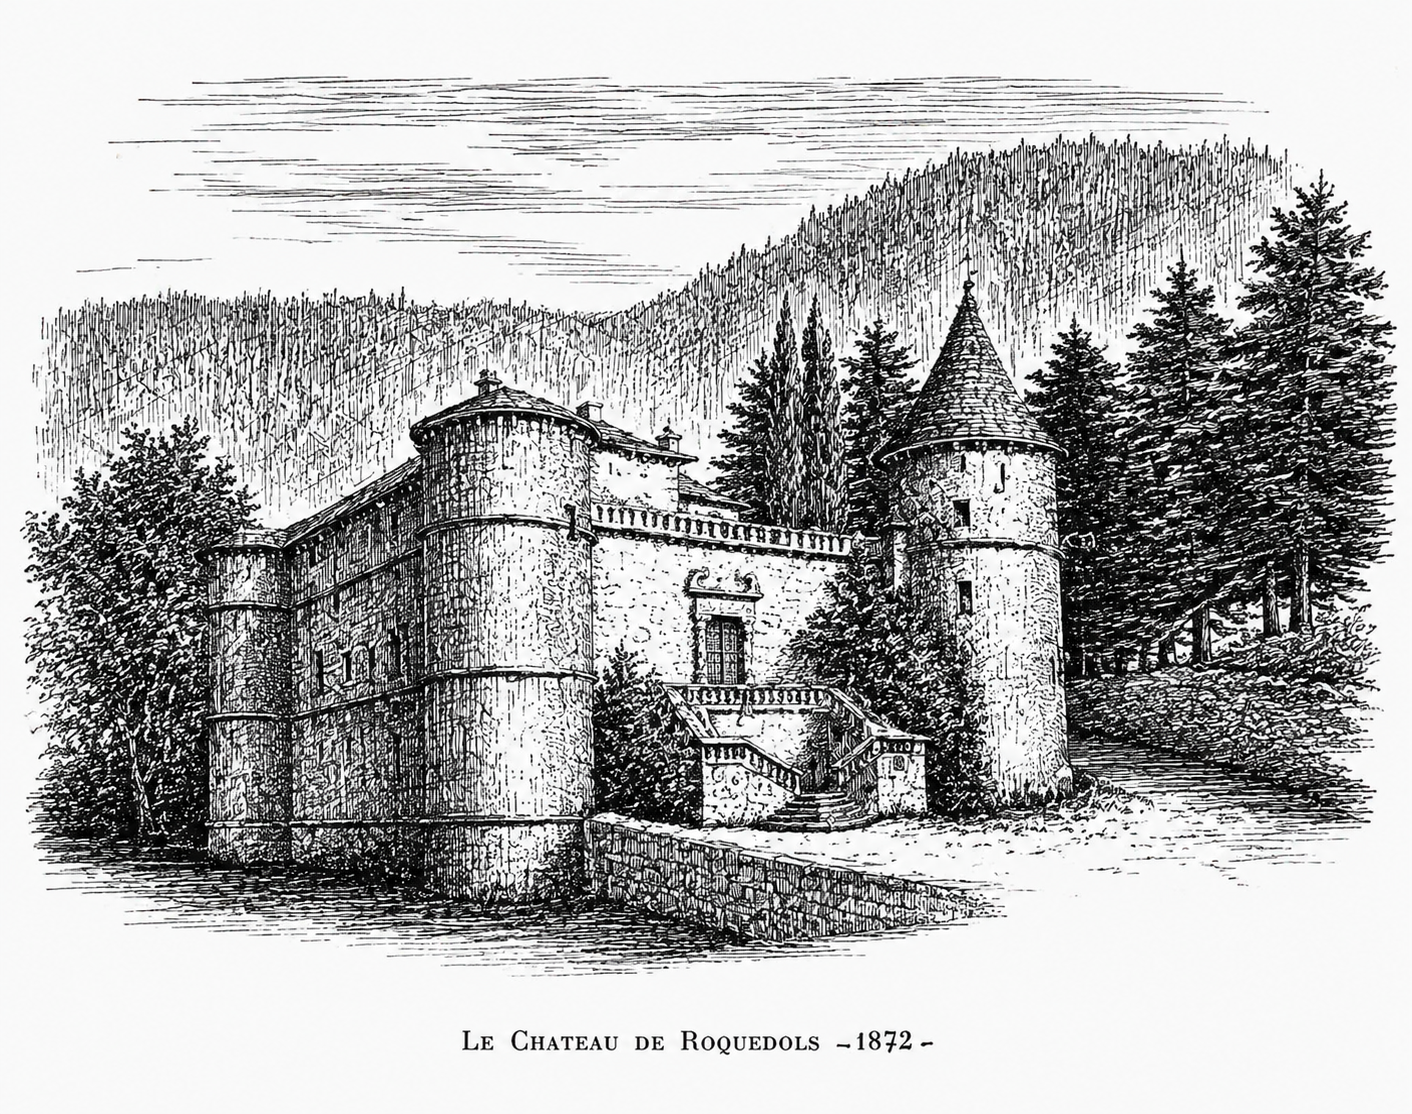
\includegraphics[width=0.92\textwidth]{imgs/028.png}
\end{center}
